\chapter{Introducción y metodología}\label{Capitulo_1}
\chapterquote{}{}

\section{Motivación}\label{I:mot}
La ciencia no avanza únicamente a través de grandes descubrimientos disruptivos, sino también mediante la acumulación de pequeños aportes que, 
en conjunto, terminan generando un impacto significativo. En esta línea, el estudio del comportamiento animal, y en especial su movimiento, 
no suele ser más que un granito de arena en el conjunto de técnicas y herramientas que los conservacionistas utilizan para proteger a las 
especies, entendiendo cómo interactúan con otros individuos, cómo utilizan su hábitat y cómo se adaptan ante el cambio del mismo. 
En el caso de la tortuga terrestre argentina, \textit{Chelonoidis chilensis}, estos aportes cobran relevancia, dado su estado de vulnerabilidad 
y el escaso conocimiento cuantitativo sobre la misma.

Nuestro objetivo general en esta tesis es estudiar y replicar el comportamiento de estas tortugas en su hábitat natural, entendiendo mejor su estrategia
de movimiento y su interacción con el entorno que las rodea. Para ello, disponemos de un conjunto de datos obtenidos mediante rastreadores de GPS,
que permiten registrar la posición de los animales a lo largo del tiempo. Adicionalmente, tomamos como principal inspiración el trabajo realizado
por C. Callenbach et al. \cite{callenbach2025}, quienes aplicaron técnicas de aprendizaje automático para clasificar los patrones de movimiento de 
tortugas en cautiverio y en su hábitat natural.

\section{Tortuga terrestre argentina: \textit{Chelonoidis chilensis}}\label{I:tortuga}

El objeto de estudio de esta tesis es la tortuga terrestre argentina, \textit{Chelonoidis chilensis}, una especie clasificada como ``En Peligro''
en la lista roja de la \textit{International Union for Conservation of Nature} (IUCN) \cite{kubisch2023chelonoidis}. Esta clasificación se ve impulsada especialmente 
por la expansión ganadera, que se encarga de segmentar y deteriorar su hábitat, y por la captura y venta ilegal de los individuos. En adición, la 
introducción de nuevos depredadores como el jabalí (\textit{Sus scrofa}) \cite{kubisch2014} pone en tensión la ya de por sí delicada población de tortugas. 
Estos reptiles son nativos de Sudamérica, abarcando gran parte de Argentina, el sur de Bolivia y el norte de Paraguay, como se observa en la Figura \ref{fig:mapa}. 

\begin{figure}[ht]
    \centering
    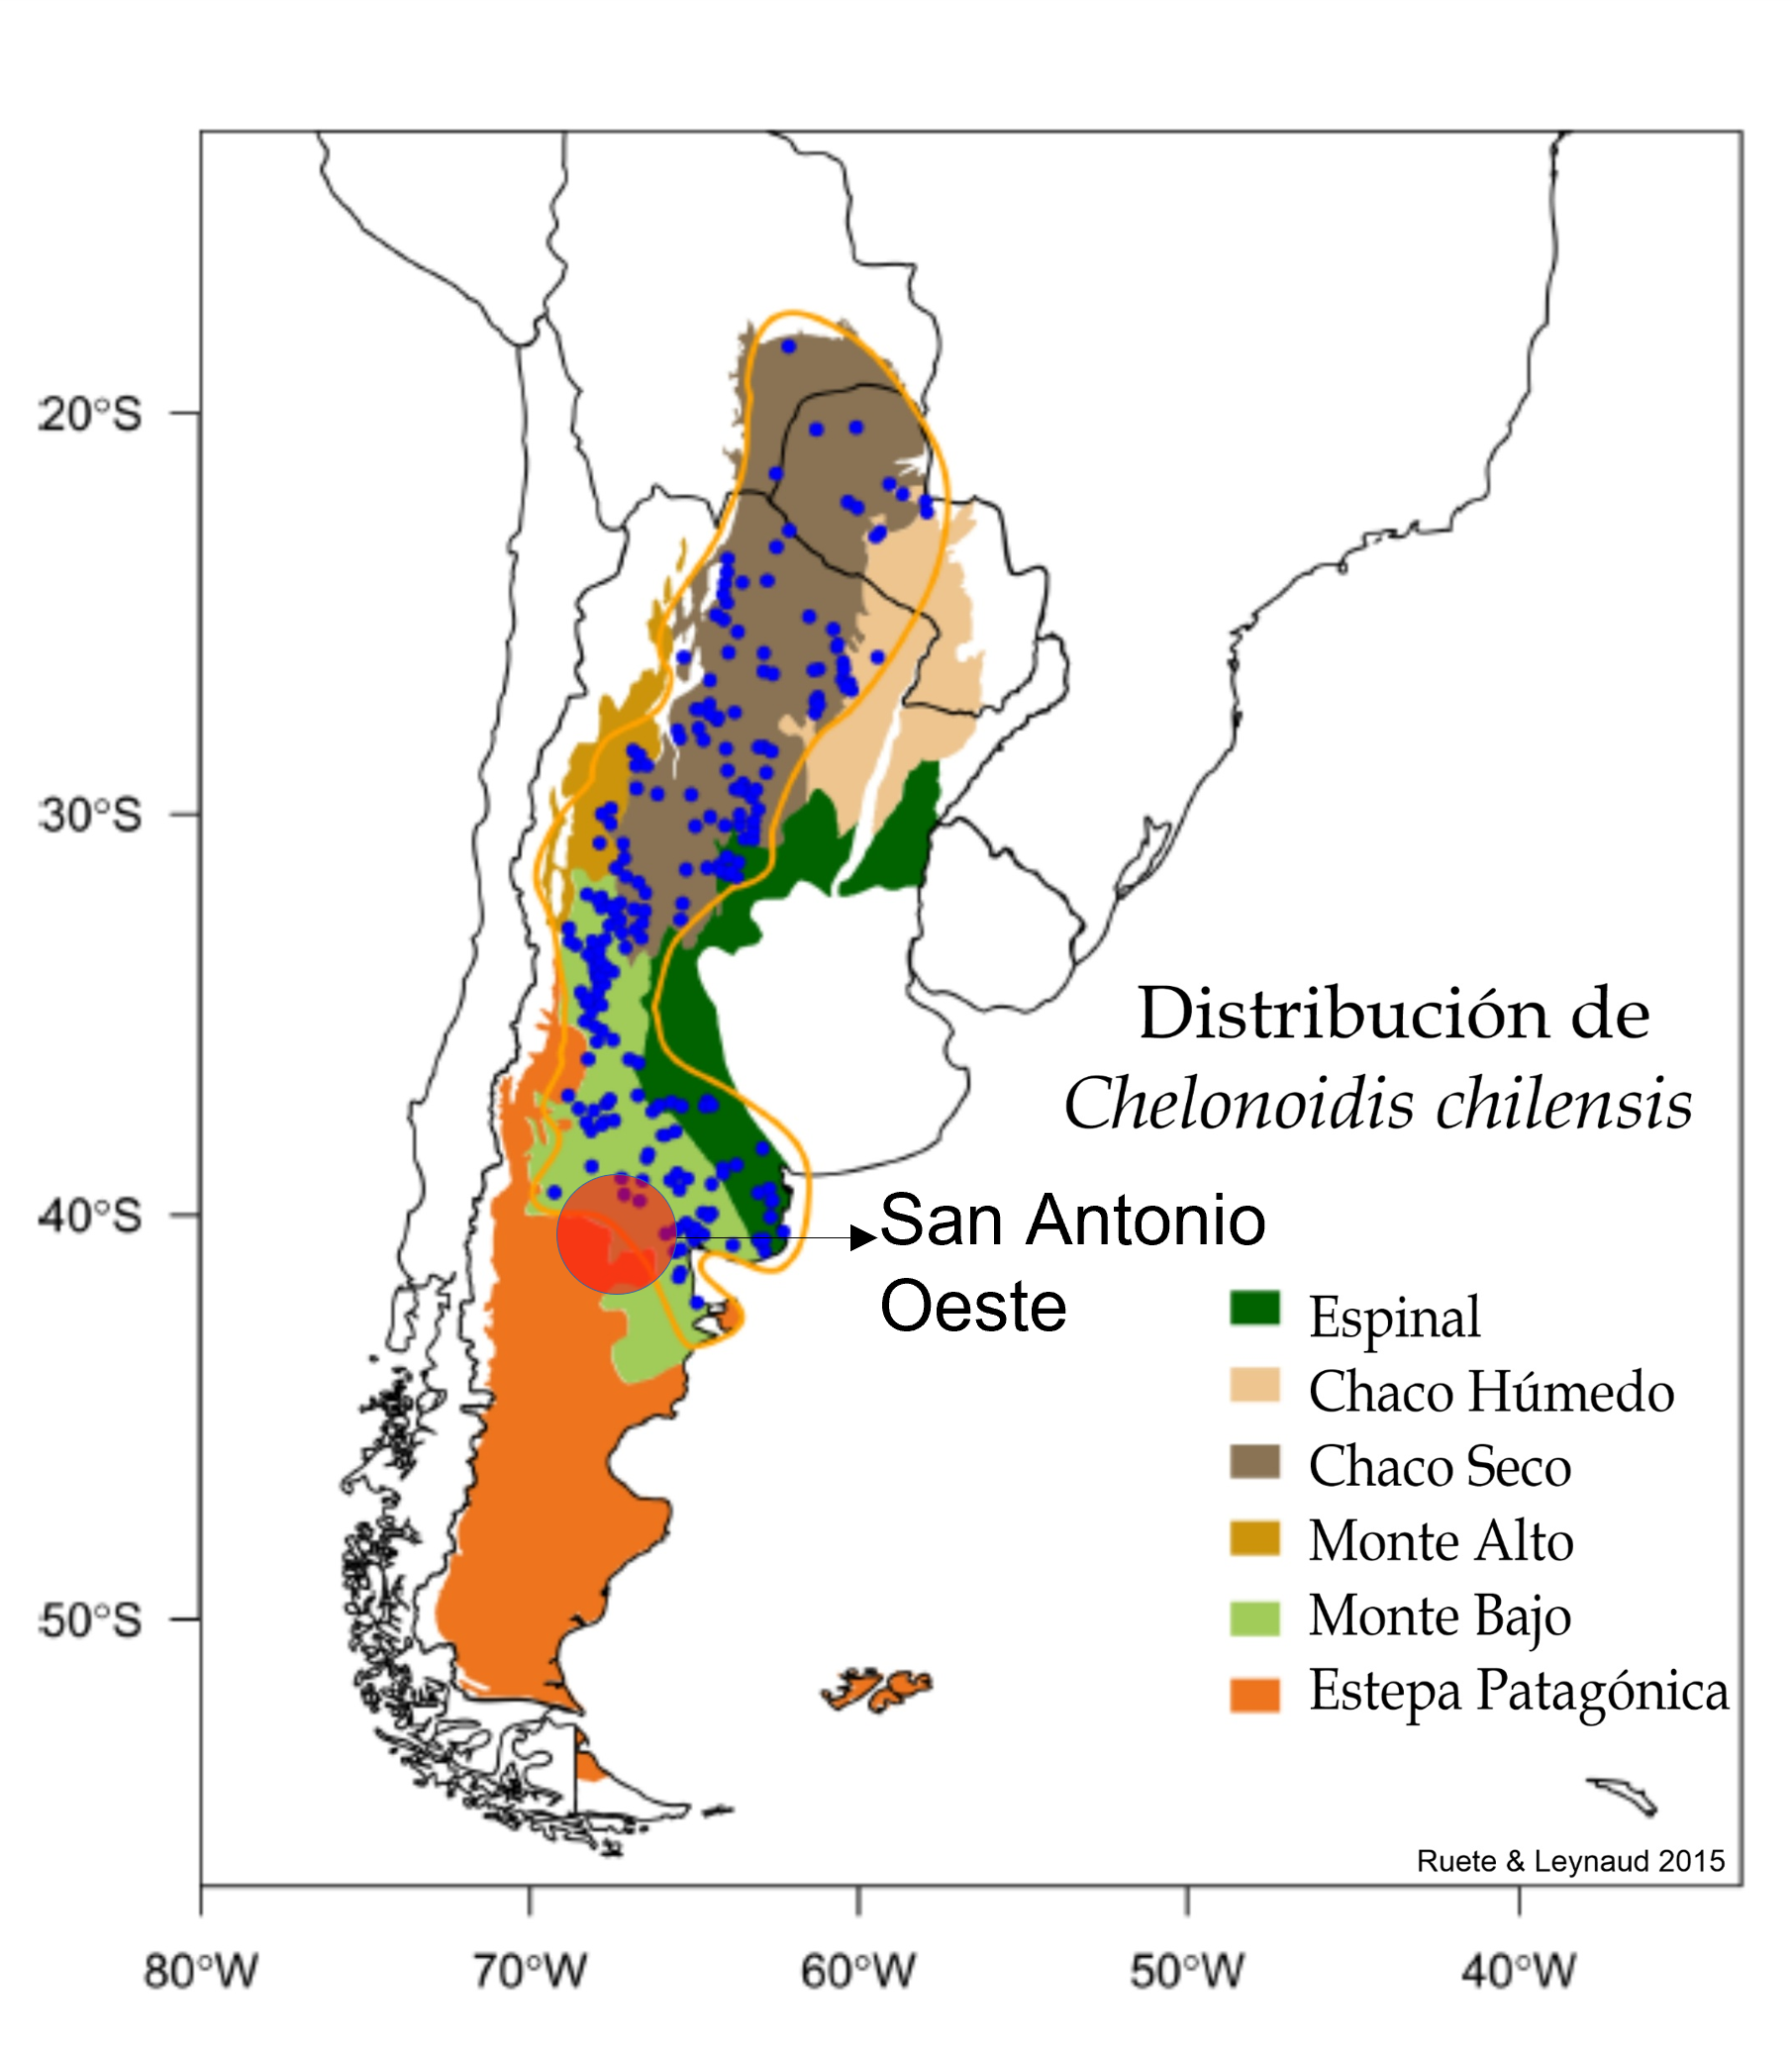
\includegraphics[scale=0.8]{figs/mapa.png}
    \caption{Distribución geográfica de la tortuga terrestre argentina, \textit{Chelonoidis chilensis}.}
    \label{fig:mapa}
\end{figure}

La especie estudiada se caracteriza por su larga esperanza de vida y su dieta herbívora. Adicionalmente, al igual que cualquier reptil, es ectoterma, 
por lo que no poseen un mecanismo interno para regular su temperatura corporal, dependiendo de la temperatura ambiental para mantener su metabolismo activo. 
Esta necesidad de depender del entorno para regular la temperatura hace que los individuos deban refugiarse en sombras provistas por la vegetación 
y reducir su actividad en condiciones de baja temperatura, dadas durante el invierno, en el que entran en brumación. Al entrar en brumación, los individuos 
se resguardan en refugios excavados en el suelo.

El trabajo de esta tesis depende de los datos obtenidos sobre una de las poblaciones más australes de la especie, ubicada a unos 20 km al norte 
de la ciudad de San Antonio Oeste, Río Negro, Argentina. Debido a la ubicación latitudinal, la variación de horas con luz solar fluctúa considerablemente
con el paso de las estaciones.

Esta especie de tortugas se encuentra dentro de la lista de animales caracterizados por un claro dimorfismo sexual, en donde las hembras son más grandes que su
contraparte masculina. Las hembras, por su parte, tienen un caparazón ventral o plastrón plano, mientras que en los machos es más cóncavo. La edad a partir de 
la cual los individuos se vuelven activos sexualmente se da entre los 10 y los 13 años. La reproducción comienza con la copulación entre individuos, para
que posteriormente la hembra seleccione el lugar donde depositará entre 2 y 4 huevos por puesta, principalmente durante los meses de enero y febrero. 
Dichos huevos suelen colocarse en un pozo de aproximadamente 10 cm y posteriormente son recubiertos por tierra. El tiempo que pueden tardar estos huevos en 
eclosionar depende de las condiciones ambientales y puede extenderse de 125 días a un año.


\section{Clasificación de comportamiento}\label{I:Charly}

Previamente mencionamos que una parte considerable de esta tesis se basa en el trabajo realizado por C. Callenbach \cite{callenbach2025} durante su tesis de licenciatura en 
el año 2025. En dicho trabajo se trabajó utilizando un dispositivo de navegación construido por el equipo de investigación del Centro Atómico Bariloche, 
el cual permitía tomar mediciones de aceleración y velocidad angular, a partir de la utilización de un acelerómetro y de un giróscopo, las cuales eran 
almacenadas en una tarjeta de memoria SD. Para evitar que el dispositivo adherido a los animales afecte su comportamiento, se suele tomar como regla 
que el mismo no debe pesar más que un $5\%$ del peso total del individuo. El dispositivo, el cual se muestra en la Figura \ref{fig:dispositivo_navegacion},
poseía un tamaño de $5 \times 8 \times 1$ cm y un peso de 44.9 g, el cual, al compararlo con el peso promedio de las tortugas de 1.5 kg, representa un $3\%$ de la masa \cite{oliva2023}.

\begin{figure}[ht]
    \centering
    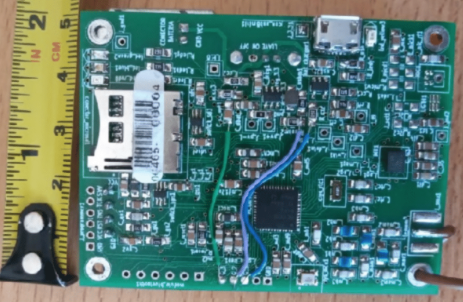
\includegraphics[width=0.75\textwidth]{dispositivo_navegacion.png}
    \caption{Dispositivo de navegación utilizado para la recolección de datos.}
    \label{fig:dispositivo_navegacion}
\end{figure}

Todos los códigos utilizados para el procesamiento de datos, entrenamiento de modelos y generación de figuras de la tesis de C. Callenbach 
están disponibles públicamente en un repositorio GitHub \cite{callenbach2025codes}.

En su trabajo logró, a partir de la utilización de herramientas de aprendizaje profundo y de mediciones de campo, clasificar el comportamiento 
de las tortugas en dos grupos (movimiento y quietud). Una vez clasificados los movimientos tiempo a tiempo, encontró que el tiempo que pasaba 
en cada uno de los estados de forma ininterrumpida seguía una distribución de ley de potencia con exponentes negativos en un rango entre $-1$ y $-2$. 
Salvo contadas excepciones para un mismo individuo, la distribución de tiempos de caminata caía de forma más abrupta que la de los tiempos de espera.
Un ejemplo de estas distribuciones se muestra en la Figura \ref{fig:distribuciones}.

\begin{figure}[ht]
    \centering
    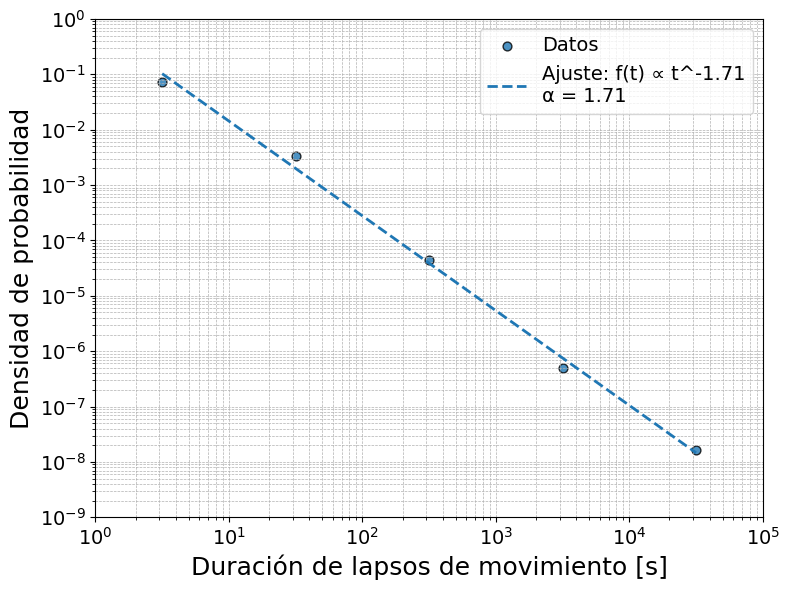
\includegraphics[width=0.45\textwidth]{distribucion_actividad_T405.png}
    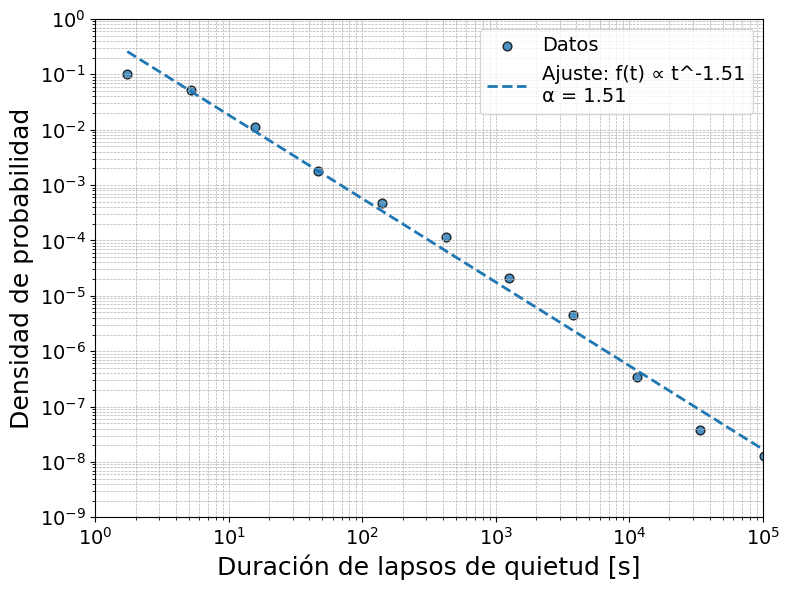
\includegraphics[width=0.45\textwidth]{distribucion_quietud_T405.png}
    \caption{Ejemplo de distribuciones de tiempos que el individuo, en este caso la tortuga T405, pasa en cada uno de los estados de forma ininterrumpida \cite{callenbach2025}.}
    \label{fig:distribuciones}
\end{figure}


\section{Datos espaciotemporales a partir de dispositivos de GPS}\label{I:GPS}

Para este trabajo utilizamos datos recolectados entre enero de 2022 y febrero de 2023. Durante estas campañas de campo se marcaba el caparazón de las tortugas para 
poder reconocerlas. Una vez identificados los individuos, se decide, teniendo en consideración la cantidad de tortugas monitoreadas y la cantidad de 
rastreadores disponibles, si se le agrega o no un dispositivo para registrar su trayectoria. Si se toma la decisión de rastrear al individuo, se le adhiere
al caparazón un dispositivo capaz de registrar las coordenadas espaciotemporales y un radiotransmisor para, al finalizar la medición, recuperar los dispositivos.
En el trabajo de tesis de M. Madile \cite{madile2023} se halla en detalle el trabajo de campaña realizado para la adquisición de datos. A continuación solo 
explicaremos el dispositivo utilizado, que sirve para el trabajo desarrollado en la presente tesis.

\subsection{Unidad de navegación}

La unidad de navegación utilizada durante la campaña para la obtención de registros espaciotemporales de la ubicación de los individuos fue el dispositivo 
comercial i-gotU GT120, mostrado en la Figura \ref{fig:igotU}. Este dispositivo posee un receptor de GPS, cuya frecuencia es ajustable mediante el 
software del fabricante. La batería del dispositivo tiene una autonomía de 7 días y su peso es de $21 g$, dicho peso representa un $1.5 \%$ del peso promedio 
de las tortugas, lo cual se encuentra dentro del margen del $5 \%$ para evitar perturbar el comportamiento. La unidad de memoria almacena posición y hora 
para cada dato adquirido, siendo accesible mediante conexión USB. 

\begin{figure}[ht]
    \centering
    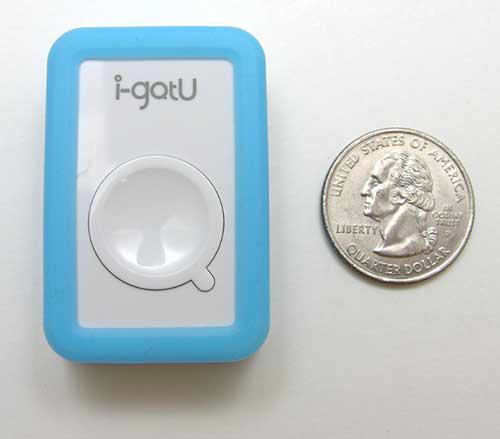
\includegraphics[width=0.45\textwidth]{IgotU.png}
    \caption{Imagen del dispositivo i-gotU, utilizado para la adquisición de datos espaciotemporales de las tortugas.}
    \label{fig:igotU}
\end{figure}

Durante esta campaña se disponía de 12 unidades de estos dispositivos, los cuales se utilizaron para medir a 6 individuos distintos, intercambiando 
los i-gotU a cada uno después de 7 días de adquisición. De esta manera se mantuvo una adquisición continua de cada una de las tortugas dado que mientras 
un dispositivo medía, su reemplazo se encontraba recargando la batería. Se programaron los dispositivos con una frecuencia de adquisición de un dato cada
15 minutos entre las 6 de la mañana y las 9 de la noche. Se evitó adquirir datos durante la noche para favorecer el ahorro de batería. Sin embargo, esta 
decisión se revirtió, tomando datos adicionales de 1am a 2am, con el objetivo de poder determinar la posición de los refugios nocturnos. La base de datos
final contó con aproximadamente 3300 horas de rastreo por tortuga.
\subsection{Errores de GPS}\label{I:ruido_noche}

Como en todo trabajo de materias de laboratorio de la facultad, lo primero que hay que hacer es caracterizar el dispositivo de medición. En este caso,
estudiamos el error de posición del GPS, para lo cual se requería de tener mediciones en donde se supiera la posición real del dispositivo. Para ello,
se usaron los pocos datos que se tenían de las mediciones nocturnas, dado que las tortugas no suelen moverse en dicho período, esto además había sido
corroborado a durante la campaña de campo. En la Figura \ref{fig:distribucion_error} se muestra la distribución de las diferencias entre dos mediciones consecutivas
del eje x y el eje y.

\begin{figure}[ht]
    \centering
    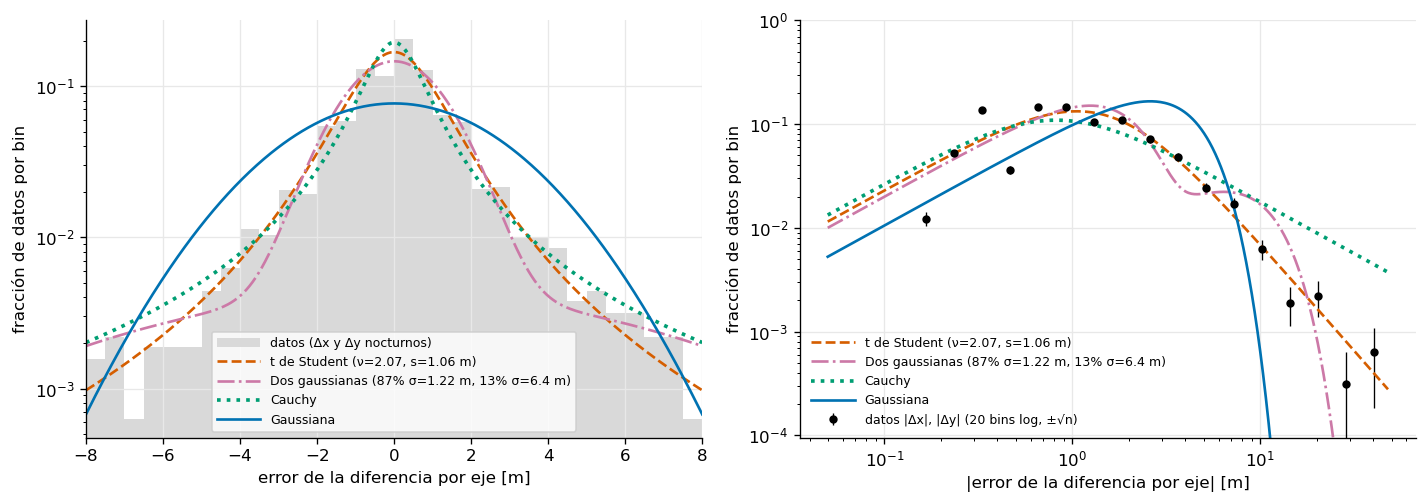
\includegraphics[width=0.95\textwidth]{Ruido noche.png}
    \caption{La figura de la izquierda muestra la frecuencia de variación de posiciones de los ejes x e y con los datos en bines logarítmicos y ajustando distintas distribuciones, 
    mientras que a la derecha se muestra la dependencia de la probabilidad de medir una desplazamiento d en 15 minutos tanto como para los datos nocturnos como para las curvas ajustadas.}
    \label{fig:distribucion_error}
\end{figure}

Se puede ver de la figura de la izquierda como no basta con un ajuste gaussiano para describir la distribución de errores, dado que los datos presentan colas más pesadas 
de las que puede replicar la función. Por ello se ajustaron otras distribuciones, como la de Cauchy, La de t de Student y una consistente en una mezcla de dos gaussianas. 
Las cuales se muestran como opciones relativamente factibles viendo dicho gráfico. Sin embargo, al ver la figura de la derecha, en donde se muestra la fracción de datos 
por bin de la variación de posición por eje. Este análisis nos permite ver que la distribución de t de Student, con $\nu=2.07$ y $s=1.06 \text{m}$ es la que mejor ajusta a los
datos. 

Esta distribución tiene una justificación natural en el contexto de un GPS. La calidad de cada medición no es siempre la misma, 
ya que depende de la cantidad y la geometría de los satélites visibles y de las reflexiones de la señal en la vegetación y el terreno. 
Por lo tanto, podemos pensar que el error de una medición en particular es gaussiano, pero con una desviación estándar $\sigma_k$ propia, 
que cambia de una medición a otra. Este comportamiento ya fue observado en otros dispositivos: para GPS de tipo Fastloc se encontró que el error por eje se describe bien con una t de Student cuyos grados de libertad aumentan con el número de satélites usados en cada medición \cite{wensveen2015}, y la t de Student también se ha usado para modelar errores de posición de otros sistemas, como Argos \cite{jonsen2005}. Como $\sigma_k$ no es fija, el error que observamos es una mezcla continua de gaussianas, y para describirla 
hace falta proponer cómo se distribuye $\sigma_k$. Una elección natural es suponer que la precisión de cada medición, $1/\sigma_k^2$, es proporcional 
a una variable $w$ que se distribuye como una $\chi^2_\nu$, es decir, como la suma de los cuadrados de $\nu$ variables gaussianas independientes de media cero y varianza uno. 
Esta es una distribución positiva, con media $\nu$, que para $\nu=2$ se reduce a una exponencial, y que permite que haya muchas mediciones con 
precisión alta y unas pocas con precisión muy baja. Con esta elección, la mezcla resulta exactamente una distribución t de Student con $\nu$ grados de libertad \cite{lange1989}. 
Explícitamente, el vector de error de una medición es
\begin{equation}
    \boldsymbol{\epsilon}=\frac{s\,\mathbf{z}}{\sqrt{w/\nu}}, \qquad \mathbf{z}\sim\mathcal{N}(0,I_2), \qquad w\sim\chi^2_\nu ,
    \label{eq:error_t}
\end{equation}
es decir, una gaussiana de varianza $\sigma_k^2=\nu s^2/w$ cuando se fija $w$. Cabe aclarar que la forma $\chi^2_\nu$ es un supuesto de modelado y no algo que 
medimos directamente: no conocemos la distribución real de $\sigma_k$ de cada medición, y lo que respalda el supuesto es que la t de Student con $\nu\approx2$ describe los datos. 
Se supone además que $x$ e $y$ comparten el mismo $w$, dado que una medición mala lo es en ambas coordenadas; 
de hecho, los tamaños de $|\Delta x|$ y $|\Delta y|$ están correlacionados (coeficiente de correlación de $0.47$), cosa que no ocurriría con dos t independientes. 
Bajo este supuesto, la distribución de la distancia $d=\sqrt{\Delta x^2+\Delta y^2}$ y su probabilidad acumulada complementaria son
\begin{equation}
    p(d)=\frac{d}{s^2}\left(1+\frac{d^2}{\nu s^2}\right)^{-(\nu/2+1)},
    \label{eq:distancia_t}
\end{equation}
cuya cola decae como $p(d)\sim d^{-(\nu+1)}$. Una consecuencia importante es que, con $\nu\approx2$, la varianza 
no está definida, por lo que no existe un único $\sigma$ que caracterice el error del GPS; este queda descrito por los parámetros $\nu$ y $s$. Así, la cola del error decae como $d^{-3}$.



%%% Local Variables: 
%%% mode: latex
%%% TeX-master: "template"
%%% End: